\section{Finite difference schemes}

\subsection{Overview}

In this section, we present explicit and implicit central finite difference schemes for solving the PDE problem in \eqref{eq:blackscholes:frontfixingmethod:inversetransform:american_options_bs_pde}. Previously, we considered the pricing problem of American options which requires solving the free boundary problem defined in \eqref{eq:blackscholes:preliminaries:american_options_pde_free_boundary_problem_full}.
Then, we presented the front fixing method as a strategy to fix the moving boundary using a change of variable. Moreover, we derived the PDE problem for call and put options that resulted from applying the Nielsen transformation suggested by \cite{nielsen_2001}, and the Company transformation suggested by \cite{company_egorova_jodar_2014}, resulting in the systems \eqref{eq:blackscholes:frontfixingmethod:inversetransform:american_options_bs_pde} and \eqref{eq:blackscholes:frontfixingmethod:logtransform:american_options_bs_pde}, respectively. In the following part, we present numerical methods for solving \eqref{eq:blackscholes:frontfixingmethod:inversetransform:american_options_bs_pde}. But before we jump into that, we define what it means to compute a numerical solution to a PDE problem.

Recall that the solution $v(x,t)$ of 
\eqref{eq:blackscholes:frontfixingmethod:inversetransform:american_options_bs_pde} is defined in the continuous region 
\begin{align*}
  \mathcal{F}: \quad & \mathcal{X} \times \mathcal{T} \\
  \mathcal{T}: \quad & [0, T] \\
  \mathcal{X}: \quad & [0, \infty)
\end{align*}
Now, we want to discretize $\mathcal{F}$ using the grid $\mathcal{G}$ with $N+1$ and $M+1$ nodes
\begin{align*}
  \mathcal{G} := \{(x_i, t_n): (i, n) \in \{0,\dots,M+1\}\times\{0,\dots,N+1\}\}
\end{align*}
where
\begin{align*}
  x_i &:= x_{\text{min}} + i\Delta x &  \qquad \text{for $i = 0,\dots, M+1$} \\
  t_n &:= t_{\text{min}} + i{\Delta t} & \qquad \text{for $i = 0,\dots, N+1$} \\
  \Delta{x} &:= \dfrac{x_{\text{max}} - x_{\text{min}}}{M+1} \\ 
  \Delta{t} &:= \dfrac{t_{\text{max}} - t_{\text{min}}}{N+1}
\end{align*}
At each node of the grid $\mathcal{G}$, we want to approximate the value function $v(x, t)$ and the optimal exercise price $\bar{S}(t)$ 
\begin{align*}
  v^{n}_i \approx v(x_i,t_n), \quad \bar{S}^{n} \approx \bar{S}(t_n)
\end{align*}
such as $\Delta{x}$ and $\Delta{t}$ decrease, the approximations $v^{n}_i$ and $\bar{S}^n$ get closer to the true value $v(x_i, t_n)$ and $\bar{S}(t_n)$, respectively. Additionally, given the PDE problem \eqref{eq:blackscholes:frontfixingmethod:inversetransform:american_options_bs_pde}, it is clear that $t_\text{min} = 0$ and $t_\text{max}=T$. Moreover, for call options, $x_\text{min} = 0$ and $x_\text{max}=1$. Likewise, for put options, $x_\text{min}=1$ and $x_\text{max}=x_\infty$ where $x_\infty$ is arbitrary large value.
\begin{figure}
  \centering
  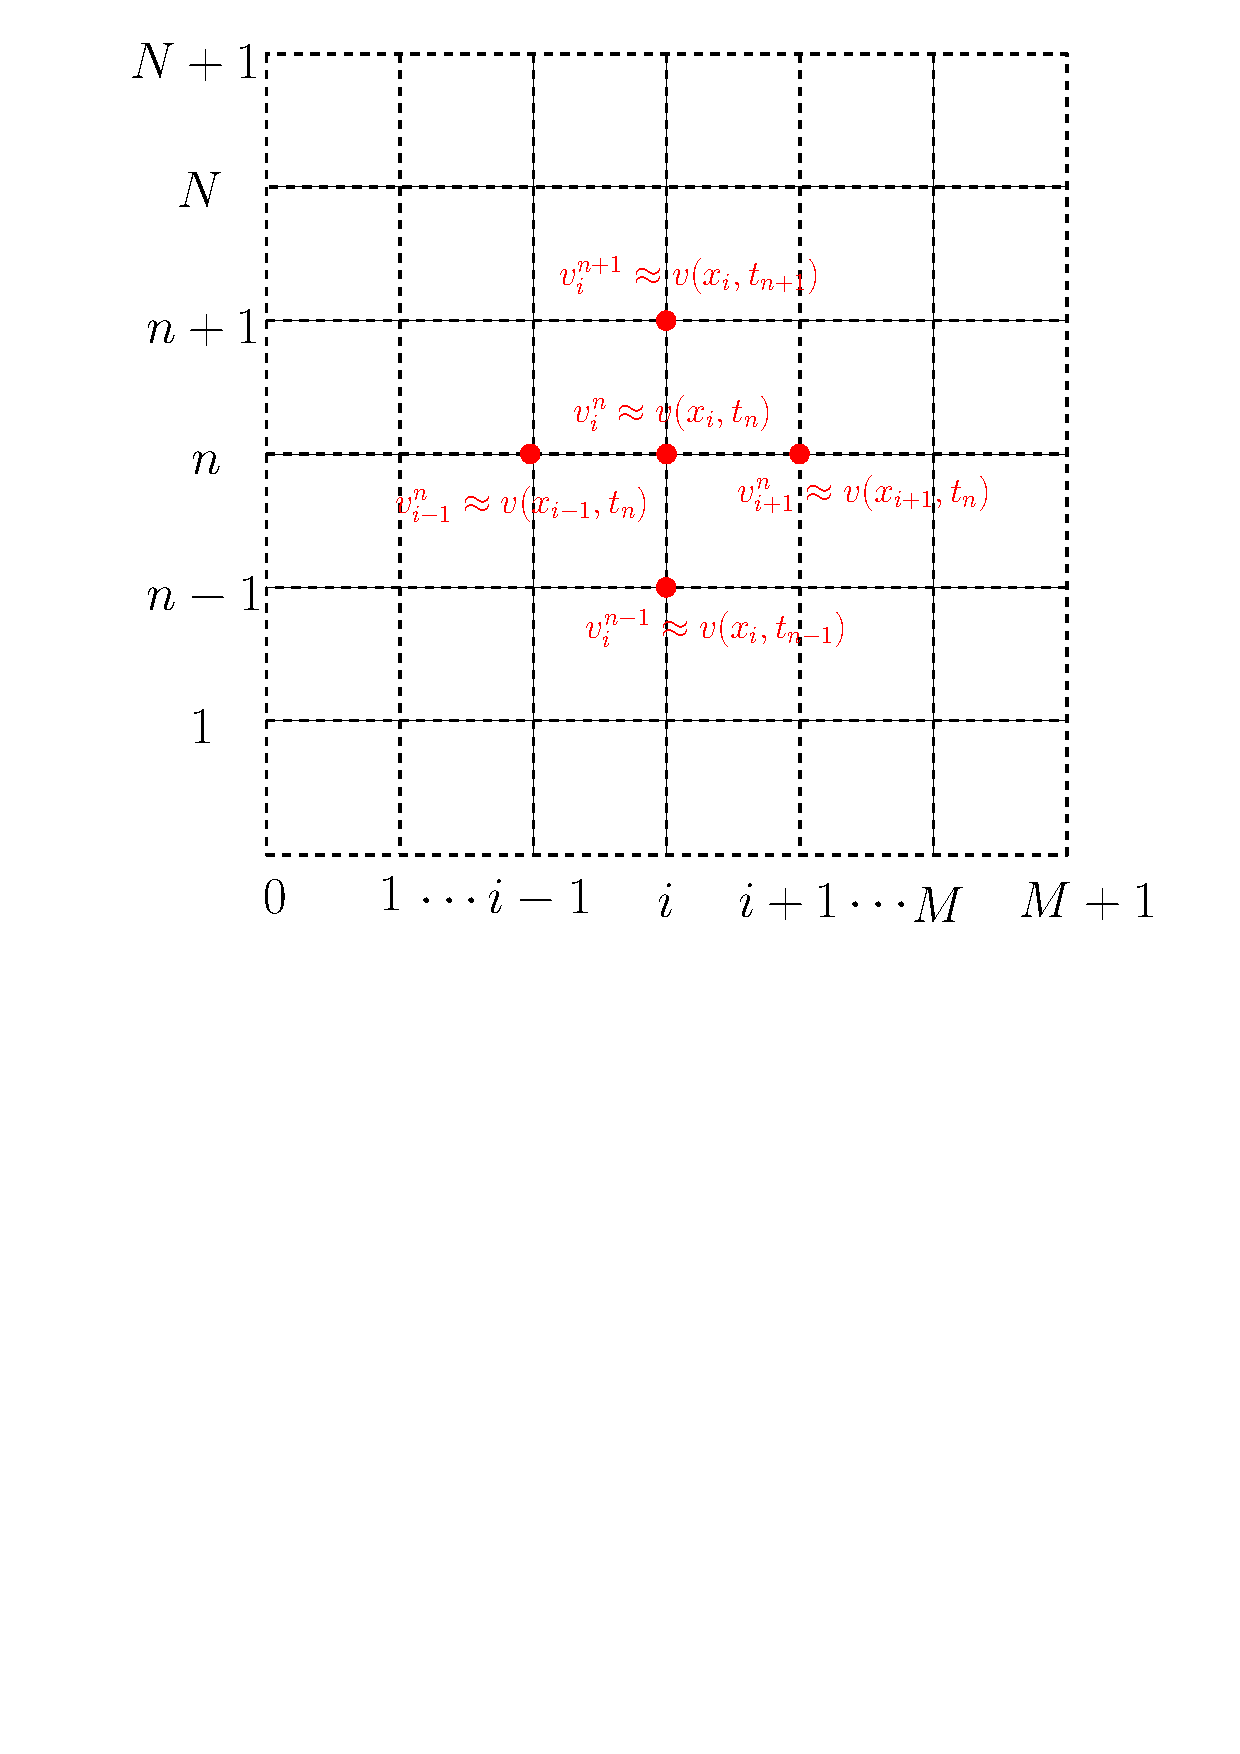
\includegraphics[scale=0.5]{chapters/chapter3/GridAproximation.pdf}
  \caption{The grid $\mathcal{G}$ and the approximation $v^{n}_{i} \approx v(x_i, t_n)$ in each node.}
  \label{fig:finitediferencesschemes:grid}
\end{figure}
\newpage
\subsection{Explicit scheme}
Generally, explicit schemes use forward finite difference at $t_n$ to approximate the temporal partial derivative and central finite difference to approximate the spatial derivative at $x_i$. However, since the problem \eqref{eq:blackscholes:frontfixingmethod:inversetransform:american_options_bs_pde} is written backward in time, we use backward finite difference at $t_{n+1}$, and a central finite difference at $x_i$.

\begin{figure}[H]
  \centering
  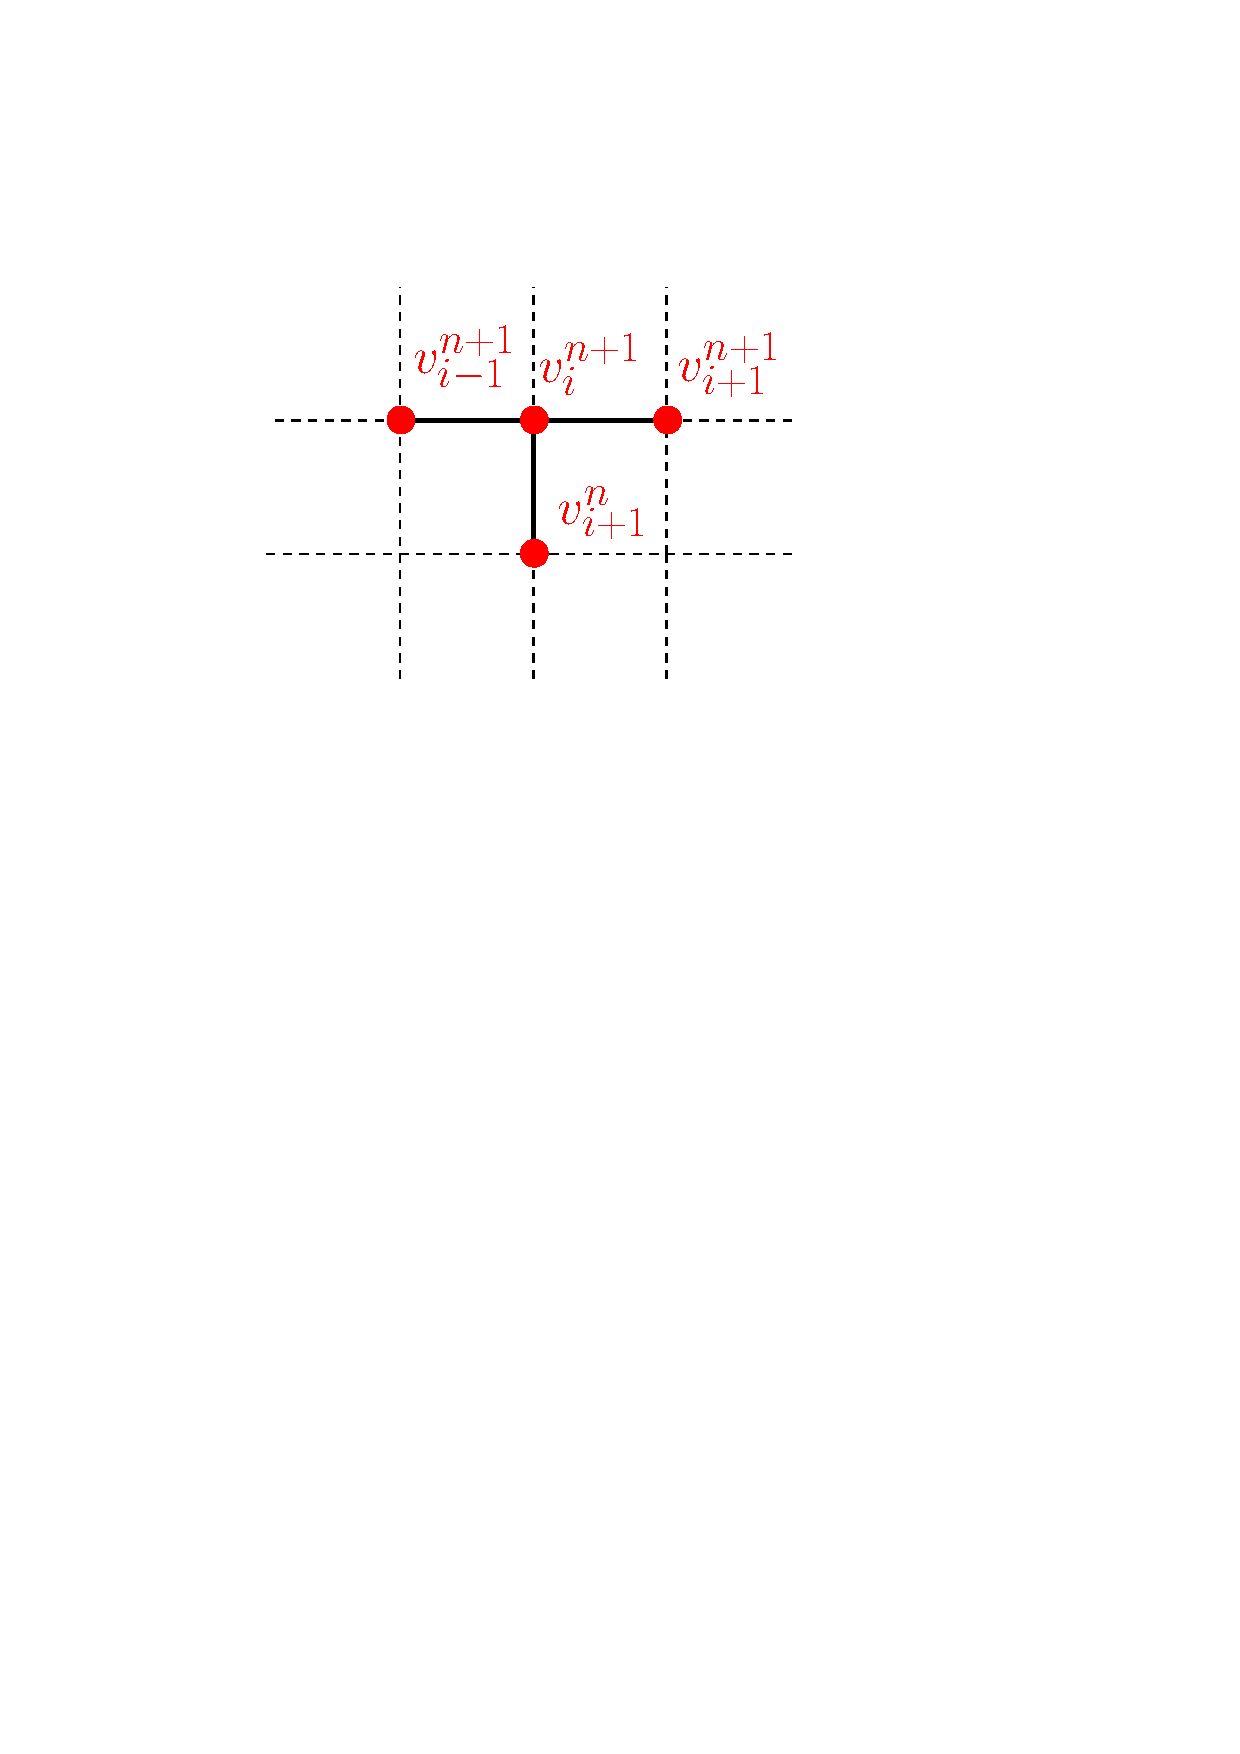
\includegraphics[scale=.8]{chapters/chapter3/ExplicitStencil.pdf}
  \caption{Stencil diagram of the explicit scheme.}
  \label{fig:finitediferencesschemes:explicit_stencil}
\end{figure}

The central finite difference for the first order and second order spatial partial derivative is given by
\begin{align}
  \label{eq:finitediferencesschemes:explicit:spatial_first_order_central_finite_difference}
  \dfrac{v^{n+1}_{i+1} - v^{n+1}_{i-1}}{2 \Delta{x}} =& \dfrac{\partial{v}}{\partial{x}}+ O(\Delta{x}^2) \qquad & \text{for $i = 1, \dots, M$} \\
  \label{eq:finitediferencesschemes:explicit:spatial_second_order_central_finite_difference}
  \dfrac{v^{n+1}_{i+1} - 2v^{n+1}_{i} + v^{n+1}_{i-1}}{\Delta{x}^2} =& \dfrac{\partial^2{v}}{\partial{x^2}}+ O(\Delta{x}^2) \qquad & \text{for $i = 1, \dots, M$}
\end{align}

As it can be observed in figure (\ref*{fig:finitediferencesschemes:explicit_stencil}), the first and second order central finite difference approximations at node $(x_i, t_{n+1})$ require to compute the difference at the nodes $(x_{i-1}, t_{n+1})$ and $(x_{i+1}, t_{n+1})$. Hence, we can only approximate the spatial partial derivative at the internal region of the grid $\mathcal{G}$ given by the nodes $(x_i, t_n)$ for $i=1,\dots,M$. Also note, that the central finite difference has second order convergence in space. In other words, as we decrease $\Delta{x}$ by one decimal place, the approximation error will decrease by two decimal places.

Analogously, the backward difference approximation at $t_{n+1}$ for $v(x, t)$ and the optimal exercise price $\bar{S}(t)$ is given by
\begin{align}
  \label{eq:finitediferencesschemes:explicit:temporal_backward_finite_difference}
  \dfrac{v^{n+1}_{i} - v^{n}_{i}}{\Delta{t}} &= \dfrac{\partial{v}}{\partial{t}}+ O(\Delta{t}) \qquad & \text{for $n = N,\dots,0$ } \\
  \label{eq:finitediferencesschemes:explicit:front_temporal_backward_finite_difference}
  \dfrac{\bar{S}^{n+1}-\bar{S}^{n}}{\Delta t} &= \bar{S}'(t) + O(\Delta{t}) \qquad & \text{for $n = N,\dots,0$ }
\end{align}
Contrary to the central finite difference, the backward finite difference approximations have first order convergence in time. While it would be desirable to have second order convergence for the temporal partial derivative approximation, it is not possible use central finite difference because we would be required to have two boundary conditions in the time axis. By combining the finite difference approximations \eqref{eq:finitediferencesschemes:explicit:spatial_first_order_central_finite_difference}, \eqref{eq:finitediferencesschemes:explicit:spatial_second_order_central_finite_difference}, \eqref{eq:finitediferencesschemes:explicit:temporal_backward_finite_difference}, and \eqref{eq:finitediferencesschemes:explicit:temporal_backward_finite_difference},the approximation of the PDE in \eqref{eq:blackscholes:frontfixingmethod:inversetransform:american_options_bs_pde} is given by 
\begin{equation*}
  \begin{split}
    \dfrac{v^{n+1}_{i} - v^{n}_{i}}{\Delta{t}} & + \dfrac{1}{2}\sigma^2 x_i^2 \dfrac{v^{n+1}_{i-1} - 2v^{n+1}_{i} + v^{n+1}_{i+1}}{(\Delta{x})^2} \\ 
     & + x_i\bigg( (r-\delta) - \dfrac{1}{\bar{S}^{n+1}}\dfrac{\bar{S}^{n+1} - \bar{S}^{n}}{\Delta{t}} \bigg)\dfrac{v^{n+1}_{i+1} - v^{n+1}_{i-1}}{2\Delta{x}} - rv^{n+1}_{i} = 0
  \end{split}
\end{equation*}
for $i = 1, \dots, M$ and $n = N, \dots, 0$. To simplify the expression above, we introduce the terms 
\begin{align*}
  \lambda &:= \dfrac{\Delta{t}}{(\Delta{x})^2} \\
  A_i &:= \dfrac{\lambda}{2}\sigma^2x^{2}_i - \dfrac{\lambda}{2}\bigg((r-\delta) - \dfrac{1}{\Delta{t}}\bigg)x_i\Delta{x} & \text{for $i = 1, \dots, M$} \\ 
  B_i &:= 1 - \lambda\sigma^2x_i^2 - r\Delta{t} & \text{for $i = 1, \dots, M$} \\
  C_i &:= \dfrac{\lambda}{2}\sigma^2x^{2}_i + \dfrac{\lambda}{2}\bigg((r-\delta) - \dfrac{1}{\Delta{t}}\bigg)x_i\Delta{x} &  \text{for $i = 1, \dots, M$} \\
  D^{n+1}_{i} &:= \dfrac{x_i}{2\Delta{x}}\dfrac{v^{n+1}_{i+1} - v^{n+1}_{i-1}}{\bar{S}^{n+1}} &  \text{for $i = 1, \dots, M$}
\end{align*}
Then, we rearrange the finite difference approximation of the PDE as 
\begin{equation}
  v^{n}_{i} - D^{n+1}_{i}\bar{S}^n = A_i v^{n+1}_{i-1} + B_{i}v^{n+1}_{i} + C_{i}v^{n+1}_{i+1}
  \label{eq:finitediferencesschemes:explicit:pde_simplified}
\end{equation}
for $i = 1, \dots, M$ and $t = N, \dots, 0$. Moreover, the PDE problem in \eqref{eq:blackscholes:frontfixingmethod:inversetransform:american_options_bs_pde} have well-defined spatial boundary conditions. For call options, the boundary conditions are located at $x=0$ and $x=1$. Similarly, for put options, the boundary conditions are located at $x=1$ and at a sufficient large $x$. However, since the $\mathcal{G}$ is defined in terms of $x_\text{min}$ and $x_\text{max}$, regardless of the option type, the boundary conditions will be always at $x_0$ and $x_{M+1}$.
\begin{subequations}
  \label{eq:finitediferencesschemes:explicit:boundary_conditions}
  \begin{align}
    \text{\textbf{Call:}} \qquad & v^{n}_{0} = 0, \qquad v^{n}_{M+1} = \bar{S}^{n} - K\\
    \text{\textbf{Put:}} \qquad & v^{n}_{0} = K - \bar{S}^{n}, \qquad v^{n}_{M+1} = 0
  \end{align}
\end{subequations}
Likewise, the terminal conditions are located at $t_{N+1}$ $i=0,\dots,M+1$
\begin{subequations}
  \label{eq:finitediferencesschemes:explicit:terminal_conditions}
  \begin{equation}
    v^{N+1}_{i} = 0, \qquad \bar{S}^{N+1} = K
  \end{equation}
\end{subequations}
Moreover, for the problem \eqref{eq:blackscholes:frontfixingmethod:inversetransform:american_options_bs_pde}, we have contact point condition \eqref{eq:blackscholes:frontfixingmethod:inversetransform:american_options_optimal_price_contact_point_condition}. The contact point condition gives the slope at $x=1$. When the option is a call option, $x=1$ correspond to $x_{M+1}$ in the grid $\mathcal{G}$. Reciprocally, for a put option, $x=1$ correspond to $x_0$. Therefore, by using backward difference at $x_{M+1}$ and forward difference at $x_0$, the contact point approximation for call and put options, respectively.
\begin{align*}
  \text{\textbf{Call:}} \qquad & \dfrac{v^{n}_{M+1} - v^{n}_{M}}{\Delta{x}} = \dfrac{\partial{v}}{\partial{x}}(1, t) + O(\Delta{x}) \\
  \text{\textbf{Put:}} \qquad & \dfrac{v^{n}_{1} - v^{n}_{0}}{\Delta{x}} = \dfrac{\partial{v}}{\partial{x}}(1, t)+ O(\Delta{x}) 
\end{align*}
Using the contact point condition, we obtain an explicit expression for $v^{n}_{M}$
\begin{subequations}
  \label{eq:finitediferencesschemes:explicit:contact_point_approximation_2}
  \begin{align}
    \text{\textbf{Call:}} \qquad& v^{n}_{M} = v^{n}_{M+1} - \Delta{x}\bar{S}^{n} = (1-\Delta{x})\bar{S}^n - K & \qquad \text{for $n = N,\dots,0$ }\\
    \text{\textbf{Put:}} \qquad& v^{n}_{1} = v^{n}_{0} - \Delta{x}\bar{S}^{n} = K - (1+\Delta{x})\bar{S}^n & \qquad \text{for $n = N,\dots,0$ }
  \end{align}    
\end{subequations}
Note that the approximation for $v^{n}_{M}$ has first order convergence in space which could degrade the global convergence of the explicit method to first order in space even if we are using central finite difference to approximate the spatial partial derivatives of $v(x,t)$. Similarly, we can obtain explicit expression for $\bar{S}^{n}$ by computing \eqref{eq:finitediferencesschemes:explicit:pde_simplified} at $x_M$ and at $x_1$ for call and put options, respectively. Then, rearranging the resulting expression in terms of $\bar{S}^n$ 
\begin{subequations}
  \label{eq:finitediferencesschemes:explicit:optimal_exercise_price_approximation}
  \begin{align}
    \text{\textbf{Call:}} \qquad& \bar{S}^{n} = \dfrac{K + A_{M}v^{n+1}_{M-1} + B_{M}v^{n+1}_{M} + C_{M}v^{n+1}_{M+1}}{(1-\Delta{x}) - D^{n+1}_{M}} \\
    \text{\textbf{Put:}} \qquad& \bar{S}^{n} = \dfrac{K - (A_{1}v^{n+1}_{0} + B_{1}v^{n+1}_{1} + C_{1}v^{n+1}_{2})}{D^{n+1}_1 + (1+\Delta{x})}
  \end{align}
\end{subequations}
for $n = N,\dots,0$. Thus, combining \eqref{eq:finitediferencesschemes:explicit:pde_simplified}, \eqref{eq:finitediferencesschemes:explicit:boundary_conditions}, 
\eqref{eq:finitediferencesschemes:explicit:terminal_conditions},
\eqref{eq:finitediferencesschemes:explicit:contact_point_approximation_2}, and \eqref{eq:finitediferencesschemes:explicit:optimal_exercise_price_approximation}, the explicit scheme of PDE problem \eqref{eq:blackscholes:frontfixingmethod:inversetransform:american_options_bs_pde} is given by
\begin{subequations}
  \label{eq:finitediferencesschemes:explicit:nielsen_system_of_equation}
  \begin{align}
    \text{\textbf{Call:}} \quad& \begin{cases}
      v^{n}_{i} - D^{n+1}_{i}\bar{S}^n = A_i v^{n+1}_{i-1} + B_{i}v^{n+1}_{i} + C_{i}v^{n+1}_{i+1} & \text{for $i = 1, \dots, M-1$ and $n = N,\dots, 0$}\\
      v^{N+1}_i = 0 & \text{for $i = 0, \dots, M+1$}  \\
      \bar{S}^{N+1} = K \\
      v^{n}_0 = 0 & \text{for $n = N, \dots, 0$} \\ 
      v^{n}_{M} = (1-\Delta{x})\bar{S}^n - K & \text{for $n = N, \dots, 0$} \\
      v^{n}_{M+1} = \bar{S}^n - K  & \text{for $n = N, \dots, 0$}
    \end{cases}\\
    \text{\textbf{Put:}} \quad&  \begin{cases}
      v^{n}_{i} - D^{n+1}_{i}\bar{S}^n = A_i v^{n+1}_{i-1} + B_{i}v^{n+1}_{i} + C_{i}v^{n+1}_{i+1} & \text{for $i = 2, \dots, M$ and $n = N,\dots,0$} \\
      v^{N+1}_i = 0 & \text{for $i = 0, \dots, M+1$} \\ 
      \bar{S}^{N+1} = K \\
      v^{n}_{0} = K - \bar{S}^{n} & \text{for $n = N, \dots, 0$} \\
      v^{n}_{1} =  K - (1+\Delta{x})\bar{S}^{n}  & \text{for $n = N, \dots, 0$} \\
      v^{n}_{M} = 0 & \text{for $n = N, \dots 0$}
    \end{cases}
  \end{align}
\end{subequations}
Finally, we formulate an algorithm for solving the system \eqref{eq:finitediferencesschemes:explicit:nielsen_system_of_equation}
\begin{algorithm}[H]
  \caption{Explicit method for call options} \label{alg:finitediferencesschemes:explicit:call_explicit_method_algorithm}
  \begin{algorithmic}
  \Ensure $\lambda \le 0.5$
  
  \For{$i = 0,\dots,M+1$} 
    \State $v^{N+1}_i = 0 $
  \EndFor
  
  \State $\bar{S}^{N+1} = K$

  \For{$i = 1,\dots,M$} 
    \State $A_i = \dfrac{\lambda}{2}\sigma^2x^{2}_i - \dfrac{\lambda}{2}\bigg((r-\delta) - \dfrac{1}{\Delta{t}}\bigg)x_i\Delta{x}$
    \State $B_i = 1 - \lambda\sigma^2x_i^2 - r\Delta{t} $
    \State $C_i = \dfrac{\lambda}{2}\sigma^2x^{2}_i + \dfrac{\lambda}{2}\bigg((r-\delta) - \dfrac{1}{\Delta{t}}\bigg)x_i\Delta{x} $
  \EndFor
  
  \For{$n = N, \dots, 0$}
    \For{$i = 1, \dots, M$}
      \State $D^{n+1}_i = \dfrac{x_i}{2\Delta{x}}\dfrac{v^{n+1}_{i+1} - v^{n+1}_{i-1}}{\bar{S}^{n+1}}$
    \EndFor
    \State $\bar{S}^n = \dfrac{K + A_{M}v^{n+1}_{M-1} + B_{M}v^{n+1}_{M} + C_{M}v^{n+1}_{M+1}}{(1-\Delta{x}) - D^{n+1}_{M}}$
    \State $v^{n}_{0} = 0$
    \State $v^{n}_{M} = (1-\Delta{x})\bar{S}^{n} - K$
    \State $v^{n}_{M+1} = \bar{S}^{n} - K$
    \For{$i = 1, \dots, M-1$}
      \State $v^{n}_{i} = A_i v^{n+1}_{i-1} + B_{i}v^{n+1}_{i} + C_{i}v^{n+1}_{i+1} + D^{n+1}_{i}\bar{S}^n$
    \EndFor
  \EndFor
\end{algorithmic}
\end{algorithm}

\begin{algorithm}[H]
  \caption{Explicit method for put options}\label{alg:finitediferencesschemes:explicit:put_explicit_method_algorithm}
  \begin{algorithmic}
  \For{$i = 0,\dots,M+1$} 
    \State $v^{N+1}_i = 0 $
  \EndFor
  \State $\bar{S}^{N+1} = K$
  \For{$i = 1,\dots,M$} 
    \State $A_i = \dfrac{\lambda}{2}\sigma^2x^{2}_i - \dfrac{\lambda}{2}\bigg((r-\delta) - \dfrac{1}{\Delta{t}}\bigg)x_i\Delta{x}$
    \State $B_i = 1 - \lambda\sigma^2x_i^2 - r\Delta{t} $
    \State $C_i = \dfrac{\lambda}{2}\sigma^2x^{2}_i + \dfrac{\lambda}{2}\bigg((r-\delta) - \dfrac{1}{\Delta{t}}\bigg)x_i\Delta{x} $
  \EndFor
  \For{$n = N, \dots, 0$}
    \For{$i = 1, \dots, M$}
      \State $D^{n+1}_i = \dfrac{x_i}{2\Delta{x}}\dfrac{v^{n+1}_{i+1} - v^{n+1}_{i-1}}{\bar{S}^{n+1}}$
    \EndFor
    \State $\bar{S}^n = \dfrac{K - (A_{1}v^{n+1}_{0} + B_{1}v^{n+1}_{1} + C_{1}v^{n+1}_{2})}{D^{n+1}_{1} + (1+\Delta{x})}$
    \State $v^{n}_{0} = K - \bar{S}^{n}$
    \State $v^{n}_{1} = K - (1+\Delta{x})\bar{S}^n$
    \State $v^{n}_{M+1} = 0$
    \For{$i = 2, \dots, M$}
      \State $v^{n}_{i} = A_i v^{n+1}_{i-1} + B_{i}v^{n+1}_{i} + C_{i}v^{n+1}_{i+1} + D^{n+1}_{i}\bar{S}^n$
    \EndFor
  \EndFor
\end{algorithmic}
\end{algorithm}

\subsection{Implicit scheme}

Analogously to the previous section, the PDE in \eqref{eq:blackscholes:frontfixingmethod:inversetransform:american_options_bs_pde} 
is approximated using forward central difference  
\begin{equation*}
  \begin{split}
    \dfrac{v^{n+1}_{i} - v^{n}_{i}}{\Delta{t}} & + \dfrac{1}{2}\sigma^2 x_i^2 \dfrac{v^{n}_{i-1} - 2v^{n}_{i} + v^{n}_{i+1}}{(\Delta{x})^2} \\ 
     & + x_i\bigg( (r-\delta) - \dfrac{1}{\bar{S}^{n}}\dfrac{\bar{S}^{n+1} - \bar{S}^{n}}{\Delta{t}} \bigg)\dfrac{v^{n}_{i+1} - v^{n}_{i-1}}{2\Delta{x}} - rv^{n}_{i} = 0
  \end{split}
\end{equation*}

Similarly to the previous section, the terms are introduced  
\begin{align}
  \alpha^{n}_{i} &:= -\dfrac{\lambda}{2}\sigma^2x^{2}_{i} + \dfrac{\lambda\Delta{x}}{2}x_{i}\bigg(r-\delta+\dfrac{\bar{S}^{n+1}-\bar{S}^n}{\Delta{t}\bar{S}^{n}}\bigg) \\
  \beta^{n}_{i} &:= 1 + \lambda\sigma^2x^{2}_{i} + r\Delta{t} \\
  \gamma^{n}_{i} &:= -\dfrac{\lambda}{2}\sigma^2x^{2}_{i} + \dfrac{\lambda\Delta{x}}{2}x_{i}\bigg(r-\delta+\dfrac{\bar{S}^{n+1}-\bar{S}^n}{\Delta{t}\bar{S}^{n}}\bigg)
\end{align}

to make the expression above more manageable. Next, the PDE approximation is rearranged as
\begin{equation*}
  \alpha^{n}_{i}v^{n}_{i-1} + \beta^{n}_{i}v^{n}_{i} + \gamma^{n}_{i}v^{n}_{i+1} = v^{n+1}_{i}
\end{equation*}

Contrary to the explicit method, there is not an explicit expression for $\bar{S^n}$. Therefore,
the PDE problem in \eqref{eq:blackscholes:frontfixingmethod:inversetransform:american_options_bs_pde}
is rewritten as
\begin{subequations}
  \begin{align}
    \begin{cases}
      \alpha^{n}_{i}v^{n}_{i-1} + \beta^{n}_{i}v^{n}_{i} + \gamma^{n}_{i}v^{n}_{i+1} = v^{n+1}_{i} & \text{for $i = 1, \dots, M-2$ and $n = N-1,\dots,0$} \\
      v^{N}_i = 0 \qquad \bar{S}^N = K & \text{for $i = 0, \dots, M$} \\
      v^{n}_0 = 0 \quad v^{n}_{M-1} = (1-\Delta{x})\bar{S}^n - K \quad v^{n}_M = \bar{S}^n - K  & \text{for $n = N-1, \dots 0$} \\
      x_{\text{min}} := 0 \quad x_{\text{max}} := 1 \\
      t_{\text{min}} := 0 \quad t_{\text{max}} := T
    \end{cases}
  \end{align}
  \begin{align}
    \begin{cases}
      \alpha^{n}_{i}v^{n}_{i-1} + \beta^{n}_{i}v^{n}_{i} + \gamma^{n}_{i}v^{n}_{i+1} = v^{n+1}_{i} & \text{for $i = 2, \dots, M-1$ and $n = N-1,\dots,0$} \\
      v^{N}_i = 0 \qquad \bar{S}^N = K & \text{for i = 0, \dots, M} \\
      v^{n}_{0} = K - \bar{S}^{n} \quad v^{n}_{1} =  K - (1+\Delta{x})\bar{S}^{n} \quad v^{n}_{M} = 0 & \text{for $n = N-1, \dots 0$} \\
      x_{\text{min}} := 1 \quad x_{\text{max}} := x_{\infty} \\
      t_{\text{min}} := 0 \quad t_{\text{max}} := T
    \end{cases}
  \end{align}
\end{subequations}

Since there is not an explicit formula for $v^{n}_{i}$ and $\bar{S}^n$, we will 
have to solve a non-linear system of equation. Let's define the vector $\mathbf{v}^n \in \mathbb{R}^{M-2}$ 
 
\begin{subequations}
  \begin{equation}
    \mathbf{v}^{n} := \begin{bmatrix}
      v^{n}_{1}, & v^{n}_{2}, & \cdots, & v^{n}_{M-2}
    \end{bmatrix}^{\text{T}}
  \end{equation}
  \begin{equation}
    \mathbf{v}^{n} := \begin{bmatrix}
      v^{n}_{2}, & v^{n}_{3}, & \cdots, & v^{n}_{M-1}
    \end{bmatrix}^{\text{T}}
  \end{equation}    
\end{subequations}

the matrix $\Lambda^{n} \in \mathbb{R}^{M-1,M-2}$ 

\begin{subequations}
  \begin{equation}
    \Lambda^{n} = \begin{bmatrix}
      \beta^{n}_{1} & \gamma^{n}_1 \\
      \alpha^{n}_{2} & \beta^{n}_{2} & \gamma^{n}_{2} \\
      & \ddots & \ddots & \ddots  \\
      & & \ddots & \ddots & \ddots  \\
      & & & \alpha^{n}_{M-3} & \beta^{n}_{M-3} & \gamma^{n}_{M-3} \\
      & & & & \alpha^{n}_{M-2} & \beta^{n}_{M-2} \\
      & & & & & \alpha^{n}_{M-2} \\
    \end{bmatrix}
  \end{equation}
  \begin{equation}
    \Lambda^{n} = \begin{bmatrix}
      \gamma^{n}_1 \\
      \beta^{n}_2 & \gamma^{n}_2 \\
      \alpha^{n}_3 & \beta^{n}_3 & \gamma^{n}_3 \\
      & \ddots & \ddots & \ddots \\
      & & \ddots & \ddots & \ddots \\
      & & & \alpha^{n}_{M-2} & \beta^{n}_{M-2} & \gamma^{n}_{M-2} \\
      & & & & \alpha^{n}_{M-1} & \beta^{n}_{M-1} \\
    \end{bmatrix}
  \end{equation}
\end{subequations}

and the vector $\mathbf{f}^{n} \in \mathbb{R}^{M-1}$

\begin{subequations}
  \begin{equation}
    \mathbf{f}^n= \begin{bmatrix}
      v^{n+1}_{1} \\
      \vdots \\
      v^{n+1}_{M-2} - \gamma^{n}_{M-2}[(1-\Delta{x})\bar{S}^{n} - K] \\
      v^{n+1}_{M-1} - \gamma^{n}_{M-1}(\bar{S}^n - K) - \beta^{n}_{M-1}[(1-\Delta{x})\bar{S}^{n} - K]
    \end{bmatrix}
  \end{equation}
  \begin{equation}
    \mathbf{f}^n= \begin{bmatrix}
      v^{n+1}_{1} - \alpha^{n}_{1}(K - \bar{S}^{n}) - \beta^{n}_{1}[K - (1+\Delta{x})\bar{S}^{n}] \\
      v^{n+1}_{2} - \beta^{n}_2[K - (1+\Delta{x})\bar{S}^{n}] \\
      v^{n+1}_{3} \\
      \vdots \\
      v^{n+1}_{M-1}
    \end{bmatrix}
  \end{equation}
\end{subequations}

Thus, the non-linear system of equations that we need to solve is

\begin{equation}
  F(\mathbf{v}^{n}, \bar{S}^{n}) = \Lambda^{n}\mathbf{v}^{n} - \mathbf{f}^n = 0
\end{equation}

By computing the Jacobian of the system, we con solve the non-linear system 
using the newton's method

\begin{equation}
  \mathbf{y}_{k+1} = \mathbf{y}_{k} - J^{-1}(\mathbf{y}_{k})F(\mathbf{y}_{k})
\end{equation}

where $y_k$ is some approximation of the solution
\begin{equation}
  \mathbf{y} = \begin{bmatrix}
    \mathbf{v}^{n} | \bar{S}^{n}
  \end{bmatrix}^{\text{T}}
\end{equation}